\section{Hypothesis Testing}

We now turn our attention to the methods to best utilize models, as well as how we can make models. \newline 
\begin{center}
\smartdiagramset{back arrow disabled=true,module minimum width=2.5cm,
module minimum height=1.5cm,text width=2.5cm,
module x sep=3.75,}
\smartdiagram[flow diagram:horizontal]{X,Model,Y}
\end{center}


\begin{center}
\smartdiagramset{back arrow disabled=true,module minimum width=2.5cm,
module minimum height=1.5cm,text width=2.5cm,
module x sep=3.75,}
\smartdiagram[flow diagram:horizontal]{State of Nature,Model,Observation}
\end{center}


\begin{center}
\smartdiagramset{back arrow disabled=true,module minimum width=2.5cm,
module minimum height=1.5cm,text width=2.5cm,
module x sep=3.75,}
\smartdiagram[flow diagram:horizontal]{Hypothesis,Model,Evidence}
\end{center}

The goal of a ``model" is to define the transition probabilities between some state of nature (or hypothesis), and some observation that we see potentially resulting from the underlying state of nature. For example, given that it is cloudy (state of nature), what is the probability that it rains (observation)? Note that we will call these transition probabilities \textbf{likelihoods}, as they represent the likelihood of seeing some observation given an underlying state of nature. We refer to the probability distribution of the states of nature as the \textbf{prior}, and we usually denote this probability distribution with the symbol \(\pi\). In our example, the prior would be the probability distribution of the different states of the sky. For example, we would have \(\pi(\textrm{cloudy}) = P(\textrm{cloudy})\), \(\pi(\textrm{sunny}) = P(\textrm{sunny})\), etc. \newline 

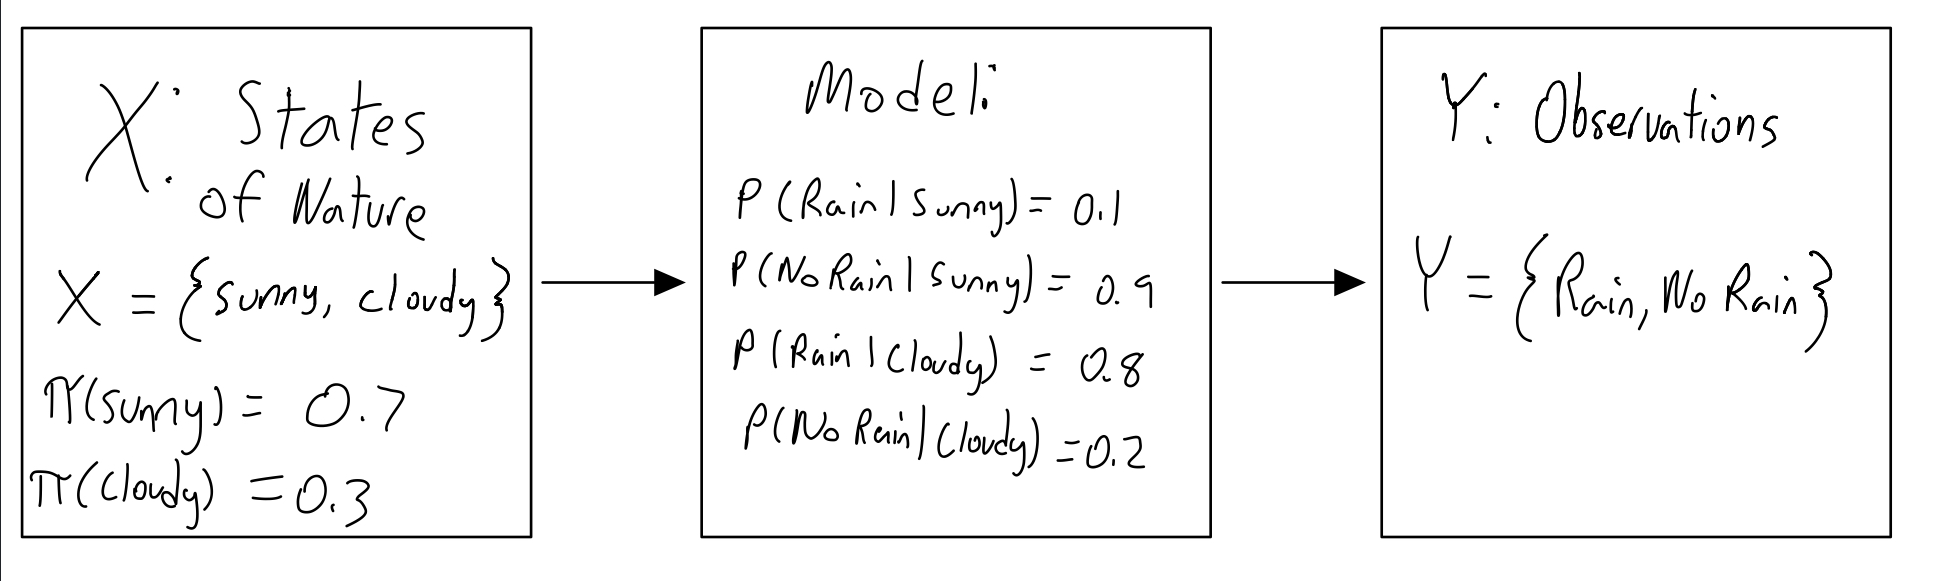
\includegraphics[width=1\textwidth]{model_diagram}

Note that our discussion has been using the phrase ``state of nature", however it will be helpful to begin thinking of this as a ``hypothesis" instead. The justification for this choice will be more clear after reading the coming sections. However, for now, whenever you see the phrase hypothesis, try thinking of it as a ``state of nature" instead if that makes more intuitive sense.
%TODO Insert diagram showing flow from state of nature -> model -> observation

  
\subsection{MAP and MLE}
Say that we are given some observation, and we would like to know under what conditions would the likelihood of observing this outcome be maximized. In other words, after seeing some evidence, we now want to know which hypothesis we believe is the most likely candidate for producing the evidence. This could be helpful if we are not able to observe the inner working of a system and are only able to observe some output of that system, but we still want to be able to make some predictions about what is going on behind the scenes. Let us now formalize our goal. Assume that the possible hypotheses lie in a set \(X\), and the possible observations lie in a set \(Y\). Given some observation \(y \in Y\), we want to find:
\begin{equation*}
  \underset{x \in X}{\argmax}\ p_{x|y}(x|y)
\end{equation*}
How can we interpret these probabilities? We know that \(\pi(x)\) is the \textit{prior} of \(x\), and it represents the probability of the hypothesis being \(x\) (no evidence observed). We can also interpret \(p_{x|y}(x|y)\) as being our updated belief about the probability of the hypothesis being \(x\) now that we have observed an observation \(y\). In other words, observing \(y\) gave us new information, and so we now want to update our beliefs on the hypotheses based on this information. Using this way of thinking is critical to understanding the utility of Bayes Law. Remember that the model gives us access to the transition probabilities between the hypotheses and the possible observations: \(p_{y|x}(y|x)\), and we know that we can relate this to \(p_{x|y}(x|y)\) using Bayes Law, and so we can can convert our goal into the following:
\begin{equation*}
  \underset{x\in X}{\argmax}\ p_{x|y}(x|y) = \underset{x \in X}{\argmax}\ \frac{p_{y|x}(y|x)p(x)}{p(y)} = \underset{x\in X}{\argmax}\  \frac{p_{y|x}(y|x)\pi(x)}{p(y)}
\end{equation*}
Note that since our goal is to find \(x\in X\) that maximizes the expression, we can ignore the denominator. This is because the denominator depends only on \(y\), and so maximizing the entire expression amounts to maximizing what we can control, which in this case is just the numerator. Therefore, to find our guess for which hypothesis caused the evidence that we saw, we define:
\begin{defn}{MAP Estimate}{}
\begin{equation*}
  \MAP (y) := \underbrace{\underset{x \in X}{\argmax}\ p_{x|y}(x|y)}_{``A\ Posteriori \ Probability"} = \underbrace{\underset{x\in X}{\argmax}\ p_{y|x}(y|x)\pi(x)}_{Computable \ with \ model}
\end{equation*}
\end{defn}

This is called the \textbf{MAP Estimate}, and it is a function of the observation. MAP stands for \textbf{Maximum A Posteriori Probability}. A Posteriori Probability refers to the ``after probability", meaning the 
updated probability distribution of the hypothesis given we observe some piece of evidence. The above equation shows how we can think about MAP. Our goal is to maximize the A Posteriori Probability, and we reduced this problem into one that we can solve by utilizing the model. \newline 

\begin{exmp}{Computing MAP}{}
Assume that we have a coin that flips heads with probability \(1/4\). Your friend (or imaginary friend) flips the coin behind your back and tells you the result. Unfortunately, your friend is very nervous (perhaps they have a 5 page essay due in 2 hours yet they chose not to begin until the last minute because they were too busy watching youtube videos all day) and occasionally tells you the opposite of the true result with probability \(2/5\). Let \(y\) represent the result that your friend tells you such that \(y=0\) represents tails and \(y=1\) represents heads. Compute \(\MAP (y=0)\) and \(\MAP (y=1)\). \newline 

We will begin with \(\MAP (y=0)\). We want to compute \(\underset{x\in X}{\argmax}\ p_{y|x}(y|x)\pi(x)\). We have: 
\begin{align*}
  &\MAP (y=0) = \\
  &\underset{x\in X}{\argmax}\ 
\begin{cases}
	p_{y|x}(hear\ tails|true\ tails)\pi(true\ tails) = 3/5(3/4)=9/20:x=true \ tails \\
	p_{y|x}(hear\ tails|true\ heads)\pi(true\ heads) = 2/5(1/4) = 2/20:x=true\ heads
\end{cases} 
\\
&= true \ tails
\end{align*}
Similarly,
\begin{align*}
  &\MAP (y=1) = \\
  &\underset{x\in X}{\argmax}\ 
\begin{cases}
	p_{y|x}(hear\ heads|true\ tails)\pi(true\ tails) = 2/5(3/4)=6/20:x=true \ tails \\
	p_{y|x}(hear\ heads|true\ heads)\pi(true\ heads) = 3/5(1/4) = 3/20:x=true\ heads
\end{cases} 
\\
&= true \ tails
\end{align*}
\newline 

This means that no matter what our nervous friend tells us, we will guess that the hypothesis (the true result of the coin flip) was actually tails. This makes some intuitive sense, since we know that our friend gives inaccurate information almost half the time, and so our best bet is to just guess the outcome that was more likely to occur. If we instead assume that our friend gives the wrong result with probability 1/5 instead, then we will get that the best estimate for the hypothesis is to believe what our friend says. This also makes intuitive sense, as decreasing the probability of hearing an incorrect result makes the evidence more valuable. This leads us to wonder if perhaps there is some threshold for this lying probability where we should believe our friend vs disregarding their evidence.


\end{exmp}


We call MAP a type of \textbf{estimator}. In particular, MAP is useful when we know the prior (the probability distribution of the hypotheses). However, what if we do not have access to this distribution? One possible solution is to assume that the prior is uniform among (us) all hypotheses: i.e. \(\pi(x) = 1/|X|\). If we try to now compute the MAP estimate using this assumption, we will be able to treat \(\pi(x)\) as a constant (since it is the same for any \(x\)), and so we will be able to pull it out of the argmax expression entirely. We will get a different type of estimate called the \textbf{MLE} or \textbf{Maximum Likelihood Estimate}:
\begin{defn}{MLE}{}
\begin{equation*}
  \MLE (y) := \underset{x \in X}{\argmax}\ p_{y|x}(y|x)
\end{equation*}
\end{defn}

This has a very nice interpretation: we will estimate the hypothesis by choosing the hypothesis that has greatest probability of producing the observed outcome, regardless of the prior distribution of the hypotheses. Note that the term we noted earlier, \textit{likelihood}, is now coming into play. With MLE, we want to maximize the likelihood (transition probability between hypothesis and evidence), which is the same thing as our ``model".

\begin{exmp}{Computing MLE}{}
Using the same example as we did for MAP, compute the MLE. \newline 

We can ignore the prior distribution, and just consider our model. In this problem, our model is the conditional probability distribution of whether or not our friend tells us the correct result. Since our friend lies with probability \(2/5\), they are more likely to be telling the truth. Thus, our MLE is to believe what our friend says since \(3/5 > 2/5\). If our friend lied with probability \(3/5\), then our MLE would become believing the opposite of what our friend tells us.
\end{exmp}

At the end of the first example, an idea of potentially finding thresholds for probabilities was mentioned. This will be a very useful technique in the coming section, so we will walk through examples of this. First, it will be useful to define a \textbf{likelihood ratio}. The purpose of this will be made more clear in the coming example.
\begin{defn}{Likelihood Ratio}{}
We define the likelihood ratio in situations where we are considering two possible hypotheses (a binary situation). We can think of this as meaning \(X = \{0, 1\}\). We define:
\begin{equation*}
  L(y) := \frac{p_{y|x}(y|x=1)}{p_{y|x}(y|x=0)}
\end{equation*}
The choice of having the likelihood for \(x=1\) in the numerator instead of \(x=0\) is just by convention.
\end{defn}


\begin{exmp}{Thresholding Intro: MLE}{}
Consider a situation our friend flips a coin (potentially biased) and reads us the result. If the result is heads, they lie about it with probability p. If the result is tails, they lie about it with probability q. We seek to compute the MLE as a function of p and q. \newline 

We have:

\begin{align*}
  &\MLE (y=0) = \\
  &\underset{x\in X}{\argmax}\ 
\begin{cases}
	p_{y|x}(hear\ tails|true\ tails) = 1-p :x=true \ tails \\
	p_{y|x}(hear\ tails|true\ heads) = p :x=true\ heads
\end{cases} 
\end{align*}
And:
\begin{align*}
  &\MLE (y=1) = \\
  &\underset{x\in X}{\argmax}\ 
\begin{cases}
	p_{y|x}(hear\ heads|true\ tails) = q :x=true \ tails \\
	p_{y|x}(hear\ heads|true\ heads) = 1-q :x=true\ heads
\end{cases} 
\end{align*}
This gives us:

\begin{align*}
  \MLE (y=0) =
  \begin{cases}
	true\ tails : p \leq 1/2 \\
	true\ heads : p > 1/2
	\end{cases} 
\end{align*}

And:

\begin{align*}
  \MLE (y=1) =
  \begin{cases}
	true\ tails : q \geq 1/2 \\
	true\ heads : q < 1/2
	\end{cases} 
\end{align*}

We can also write this in terms of the likelihood ratio by noticing that \(L(y=0) = p/(1-p)\), and similarly \(L(y=1) = (1-q)/q\). This gives us the equivalent formulation:

\begin{align*}
  \MLE (y=0) =
  \begin{cases}
	true\ tails : L(y=0) \leq 1 \\
	true\ heads : L(y=0) > 1
	\end{cases} 
\\
  \MLE (y=1) =
  \begin{cases}
	true\ tails : L(y=1) \leq 1 \\
	true\ heads : L(y=1) > 1
	\end{cases} 
\end{align*}

And finally, we can reduce this to:

\begin{align*}
  \MLE (y) =
  \begin{cases}
	0 : L(y) \leq 1 \\
	1 : L(y) > 1
	\end{cases} 
\end{align*}

If this formulation is not immediately clear, try plugging in some values for p and q to convince yourself that these are two equivalent formulations.

\end{exmp}


\begin{exmp}{Thresholding Intro: MAP}{}
Consider a situation our friend flips a coin (potentially biased) and reads us the result. If the result is heads, they lie about it with probability p. If the result is tails, they lie about it with probability q. We seek to compute the MLE as a function of p and q. \newline 

Note that since we did not specify the bias of the coin, we will have to give a name to the bias. For this, we notice that the bias of the coin is the prior distribution, and so we will denote the bias by \(\pi(0)\) and \(\pi(1)\). Since this is Bernoulli, we have that \(\pi(1) = 1- \pi(0)\). Note that \(x = 0\) corresponds to the case \(true \ tails\), and \(x = 1\) corresponds to the case \(true \ heads\).


\begin{align*}
  &\MAP (y=0) = \\
  &\underset{x\in X}{\argmax}\ 
\begin{cases}
	p_{y|x}(hear\ tails|true\ tails)\pi(true\ tails) = (1-p) \cdot \pi(0) : x=true \ tails \\
	p_{y|x}(hear\ tails|true\ heads)\pi(true\ heads) = p \cdot \pi(1) : x=true\ heads
\end{cases} 
\end{align*}
Similarly,
\begin{align*}
  &\MAP (y=1) = \\
  &\underset{x\in X}{\argmax}\ 
\begin{cases}
	p_{y|x}(hear\ heads|true\ tails)\pi(true\ tails) = q \cdot\pi(0):x=true \ tails \\
	p_{y|x}(hear\ heads|true\ heads)\pi(true\ heads) = (1-q)\cdot\pi(1) :x=true\ heads
\end{cases} 
\end{align*}

Thus, we have:

\begin{align*}
  \MAP (y=0) =
  \begin{cases}
	true\ tails : (1-p) \cdot \pi(0) \geq p \cdot \pi(1) \\
	true\ heads : (1-p) \cdot \pi(0) < p \cdot \pi(1)
	\end{cases} 
\end{align*}

And:

\begin{align*}
  \MAP (y=1) =
  \begin{cases}
	true\ tails : q \cdot \pi(0) \geq (1-q) \cdot \pi(1) \\
	true\ heads : q \cdot \pi(0) < (1-q) \cdot \pi(1)
	\end{cases} 
\end{align*}

Rearranging the inequalities so that we can rewrite in terms of \(L(y=0)\) and \(L(y=1)\) gives:

\begin{align*}
  \MAP (y=0) =
  \begin{cases}
	true\ tails : L(y=0) \leq \pi(0) / \pi(1) \\
	true\ heads : L(y=0) > \pi(0) / \pi(1)	\end{cases} 
\\
  \MAP (y=1) =
  \begin{cases}
	true\ tails : L(y=1) \leq \pi(0) / \pi(1) \\
	true\ heads : L(y=1) > \pi(0) / \pi(1)
	\end{cases} 
\end{align*}
This can finally be reduced to:
\begin{align*}
  \MAP (y) =
  \begin{cases}
	0 : L(y) \leq \pi(0) / \pi(1) \\
	1 : L(y) > \pi(0) / \pi(1)	
	\end{cases} 
\end{align*}


\end{exmp}

As we can see from the last two examples, for a given problem we are able to find the thresholds for which our estimates change based entirely on the likelihood ratio. We will continue to make use of the likelihood ratio in the next section.



\subsection{Binary Hypothesis Testing}
Binary hypothesis testing handles situations where \(|X| = 2\), which means we can equivalently view our set of hypotheses as being \(X = \{0, 1\}\). By convention, we say that \(x=0\) is the \textbf{null hypothesis}, and \(x=1\) is the \textbf{alternate hypothesis}. Our goal is to create a ``decision rule" or ``test" that tells us which hypothesis we should guess if we are given an observation. In other words, a decision rule is a function \(\hat{X}:Y \to\{0, 1\}\) (a function that maps an observation to either \(0\) or \(1\)). 
\begin{defn}{Decision Rule}{}
If \(X = \{0, 1\}\) is our set of hypotheses, and \(Y\) is our set of evidence, then a function \(\hat{X}:Y \to\{0, 1\}\) is called a \textbf{decision rule}.
\end{defn}

With any decision rule, there are two possible errors that can occur. We define them below:

\begin{defn}{Type I and Type II Errors}{}
Type I Error = False Positive: \(P(\hat{X} = 1 |x=0)\) (Probability our decision rule outputs 1, but the true hypothesis is 0) \newline 

Type II Error = False Negative: \(P(\hat{X} = 0 |x=1)\) (Probability our decision rule outputs 0, but the true hypothesis is 1) \newline 
\end{defn}

An optimal test would be able to minimize both of these errors, however minimizing two quantities simultaneously is difficult to quantify (how do we weight the value of each error type? What if minimizing type I is more important than minimizing type II? etc.). Thus, to search for an ``optimal" test we will rephrase our optimization objective. We will first pick some \(\beta \geq 0\) and say that we will minimize the rate of type II errors subject to the constraint that the rate of type I errors is less than or equal to \(\beta\). In other words, once we have picked some constant \(\beta \geq 0\), we limit our space of all possible decision rules to a smaller space of all decision rules that achieve a type I error rate that is smaller than or equal to \(\beta\). Of this smaller set of decision rules, we wish to find the one that minimizes the rate of type II errors. Mathematically, let \(S\) denote the set of all possible decision rules. Let \(S_\beta\) be the set of decision rules that achieve a type I error rate less than or equal to beta, i.e.: \(S_\beta = \{\hat{X} \in S : \underbrace{P(\hat{X} = 1 |x=0)}_{Type\ I\ Error\ Rate} \leq \beta\}\). Then, we define our optimal test:
\begin{defn}{Optimal Decision Rule}{}
\begin{equation*}
  \hat{X}^* = \underset{\hat{X}\in S_\beta}{\argmin}\ \underbrace{P(\hat{X} = 0 |x=1)}_{Type\ II\ Error\ Rate}
\end{equation*}
\end{defn}

The question remains if there is a way to more easily find this optimal decision rule in \(S_\beta\), as it doesn't seem like a good time to consider every single possible decision rule. The following result gives us a very elegant characterization:
\begin{thm}{Neyman-Pearson Lemma}{neyman_pearson}
Given \(\beta \in [0,1]\), the optimal decision rule is a (randomized) threshold test:
\begin{equation*}
  \hat{X}_\beta (y) =
  \begin{cases}
  	1 \textrm{ if \(L(y) > \lambda\)} \\
  	0 \textrm{ if \(L(y) < \lambda\)} \\
  	\Bern{\gamma} \textrm{ if \(L(y) = \lambda\)}
  	
  \end{cases}
\end{equation*}
Where \(\lambda, \gamma\) are chosen so that:
\begin{equation*}
  \underbrace{P(\hat{X}_\beta (y) = 1 | x = 0)}_{Type\ I\ Error\ Rate} = \beta
\end{equation*}

\(\hat{X}_\beta (y)\) is  called the ``Neyman-Pearson Rule", and it is the most ``powerful" test (i.e. the test that minimized the type II error) subject to the constraint that \(P(\textrm{Type I Error}) \leq \beta\)


\end{thm}



 






